% !TEX TS-program = pdflatex
% !TEX encoding = UTF-8 Unicode

% This is a simple template for a LaTeX document using the "article" class.
% See "book", "report", "letter" for other types of document.

\documentclass[11pt]{article} % use larger type; default would be 10pt

\usepackage[utf8]{inputenc} % set input encoding (not needed with XeLaTeX)

%%% Examples of Article customizations
% These packages are optional, depending whether you want the features they provide.
% See the LaTeX Companion or other references for full information.

%%% PAGE DIMENSIONS
\usepackage{geometry} % to change the page dimensions
\geometry{a4paper} % or letterpaper (US) or a5paper or....
% \geometry{margin=2in} % for example, change the margins to 2 inches all round
% \geometry{landscape} % set up the page for landscape
%   read geometry.pdf for detailed page layout information

\usepackage{graphicx} % support the \includegraphics command and options

% \usepackage[parfill]{parskip} % Activate to begin paragraphs with an empty line rather than an indent

%%% PACKAGES
\usepackage{booktabs} % for much better looking tables
\usepackage{array} % for better arrays (eg matrices) in maths
\usepackage{paralist} % very flexible & customisable lists (eg. enumerate/itemize, etc.)
\usepackage{verbatim} % adds environment for commenting out blocks of text & for better verbatim
\usepackage{subfig} % make it possible to include more than one captioned figure/table in a single float
% These packages are all incorporated in the memoir class to one degree or another...

%%% HEADERS & FOOTERS
\usepackage{fancyhdr} % This should be set AFTER setting up the page geometry
\pagestyle{fancy} % options: empty , plain , fancy
\renewcommand{\headrulewidth}{0pt} % customise the layout...
\lhead{}\chead{}\rhead{}
\lfoot{}\cfoot{\thepage}\rfoot{}
\usepackage{multicol}
\usepackage{subfig}
%%% SECTION TITLE APPEARANCE
\usepackage{sectsty}
\allsectionsfont{\sffamily\mdseries\upshape} % (See the fntguide.pdf for font help)
% (This matches ConTeXt defaults)
\usepackage{graphicx}
\usepackage{hyperref}
\usepackage{listings}
\usepackage{color}
\usepackage{floatrow}
\usepackage[section]{placeins}
\definecolor{dkgreen}{rgb}{0,0.6,0}
\definecolor{gray}{rgb}{0.5,0.5,0.5}
\definecolor{mauve}{rgb}{0.58,0,0.82}
\usepackage{afterpage} 
\lstset{frame=tb,
  language=Python,
  aboveskip=3mm,
  belowskip=3mm,
  showstringspaces=false,
  columns=flexible,
  basicstyle={\tiny\ttfamily},
  numbers=none,
  numberstyle=\tiny\color{gray},
  keywordstyle=\color{blue},
  commentstyle=\color{dkgreen},
  stringstyle=\color{mauve},
  breaklines=true,
  breakatwhitespace=false
  tabsize=3
}
%%% ToC (table of contents) APPEARANCE
\usepackage[nottoc,notlof,notlot]{tocbibind} % Put the bibliography in the ToC
\usepackage[titles,subfigure]{tocloft} % Alter the style of the Table of Contents
\renewcommand{\cftsecfont}{\rmfamily\mdseries\upshape}
\renewcommand{\cftsecpagefont}{\rmfamily\mdseries\upshape} % No bold!
\usepackage{amsmath}
%%% END Article customizations

%%% The "real" document content comes below...

\title{Project 1}
\author{Alex Dombos, Samuel Lipschutz, Charles Loelius}
%\date{} % Activate to display a given date or no date (if empty),
         % otherwise the current date is printed 

\begin{document}
\maketitle

\section{$^{11}Be$ Structure}


Based on a naive view of the shell model of the nucleus, the expected configuration of the 7 neutrons in the ground state of beryllium-11 to be $(1s_{\frac{1}{2}})^{2}(1p_{\frac{3}{2}})^{4}(1p_{\frac{1}{2}})^{1}$. However, for certain nuclei the neutron configuration may depend on the proton configuration (reference 1). In the case of beryllium-11, the 1s$_{\frac{1}{2}}$ orbit is pushed down below the 1p$_{\frac{1}{2}}$ orbit. Therefore, the correct configuration for the neutrons is $(1s_{\frac{1}{2}})^{2}(1p_{\frac{3}{2}})^{4}(2s_{\frac{1}{2}})^{1}$.

Centrifugal barrier...

A (t,p) reaction was used to investigate the excited states of beryllium-11 (reference 1 and 2). Based on the $^{9}$Be(t,p)$^{11}$Be reaction, the excited states from experiment are found in Table 1.

\begin{table}[ht] 
\caption{$^{11}$Be levels observed in the $^{9}$Be(t,p)$^{11}$Be reaction}% title of Table 
\centering % used for centering table 
\begin{tabular}{c c c c c} % centered columns (4 columns) 
\hline\hline %inserts double horizontal lines 
$E_{x}$ (MeV $\pm$ keV) & Width (keV) & Configuration & $J^{\pi}$ \\ [0.5ex] % inserts table 
%heading 
\hline % inserts single horizontal line 
0                           &                           & $^{10}$Be($0^{+}$)$\otimes$(2s$_{\frac{1}{2}}$)$_{\nu}$ & $\frac{1}{2}^{+}$ \\ [1ex] % inserting body of the table 
0.320 $\pm$ 2   &                           &                                                                                                         & $\frac{1}{2}^{-}$ \\ [1ex]
1.784 $\pm$ 4   & 104 $\pm$ 21 & $^{10}$Be($0^{+}$)$\otimes$(1d$_{\frac{5}{2}}$)$_{\nu}$ & $\frac{5}{2}^{+}$ \\ [1ex]
2.642 $\pm$ 9   & 228 $\pm$ 21 &                                                                                                         & $\frac{3}{2}^{-}$ \\ [1ex]
3.398 $\pm$ 6   & 104 $\pm$ 17 & $^{9}$Be($0^{+}$)$\otimes$(sd)$^{2}_{0^{+}}$                    & $\frac{3}{2}^{-}$ \\ [1ex]
3.888 $\pm$ 1   &                           & $^{10}$Be($2^{+}$)$\otimes$(s$\frac{1}{2}$)                        & $\frac{3}{2}^{+}$ \\ [1ex] 
3.955 $\pm$ 1   &                           & $^{9}$Be($0^{+}$)$\otimes$(sd)$^{2}_{2^{+}}$                    & $\frac{3}{2}^{-}$ \\ [1ex]  
5.255 $\pm$ 3   &                           & $^{9}$Be($0^{+}$)$\otimes$(sd)$^{2}_{2^{+}}$                    & $\frac{5}{2}^{-}$ \\ [1ex]
5.849 $\pm$ 10 & 139 $\pm$ 17 & $^{9}$Be($0^{+}$)$\otimes$(sd)$^{2}_{2^{+}}$                    & $\frac{1}{2}^{-}$ \\ [1ex] % [1ex] adds vertical space 
\hline %inserts single line 
\end{tabular} 
\label{table:nonlin} % is used to refer this table in the text 
\end{table} 

For example, the ground state occurs when the beryllium-10 core is coupled to a 2s$_\frac{1}{2}$ neutron (meaning the angular momentum quantum number, L, is zero) and has a spin and parity of $J^{\pi}=\frac{1}{2}^{+}$; the first excited state occurs 0.320 MeV above the ground state and had a spin and parity of $J^{\pi}=\frac{1}{2}^{-}$; the second excited state occurs when the beryllium-10 core is coupled to a 1d$_{\frac{5}{2}}$ neutron (meaning the angular momentum quantum number, L, is two), at 1.784 MeV, and had a spin and parity of $J^{\pi}=\frac{5}{2}^{+}$. The second excited state was identified as a resonance that had a width of 104 keV.
\section{Scattering Equations for  $n-^{10}Be $ with Arbitrary L}


\subsection{Radial Scattering Equations}
We can write Schrodinger's equations as 
\begin{equation}
H\psi=E\psi
\end{equation}

Now using a basic separation of variables and have that in spherical coordinates with azimuthal symmetry(which we have in this instance)\\

\begin{equation}
\psi=\Sigma_{l=0}^\infty (2L+1)i^LP_l(\cos\theta)\frac{1}{kr}\chi_L(r)
\end{equation}

We can then just consider the r equation, leaving us with:

\begin{equation}
(-\frac{\hbar^2}{2\mu}(\frac{d^2}{dr^2}-\frac{L(L+1)}{r^2})+V(r)-E)\chi_L(r)=0
\end{equation}

Where we can then plug in for V:\\
\begin{equation}
(-\frac{\hbar^2}{2\mu}(\frac{d^2}{dr^2}-\frac{L(L+1)}{r^2})+\frac{V_0}{1+e^{\frac{r-R_{ws}}{a_{ws}}}}-E)\chi_L(r)=0
\end{equation}

We can represent this as:\\

\begin{equation}
\boxed{\chi''(r)=\frac{2\mu}{\hbar^2}(\frac{V_0}{1+e^{\frac{r-R_{ws}}{a_{ws}}}}-E)\chi+\frac{L(L+1)}{r^2}\chi}
\end{equation}
\subsection{Scattering Boundary Conditions}
Now, if we plug in numbers for all of the constants, and make some assumptions for E and L, we are able to solve this numerically, if in addition we provide some sort of boundary conditions. We know that in order to prevent the terms from blowing up, this means that we need $\chi_L(0)=0$, which is one such condition. We also need to have, for an elastic collision, the condition that at infinity we should expect the wavefunction to return to the form $e^{ikr+\delta}$. This can be written as at some chosen distance $a$, where we would want $e^{ika+\delta}$, noting tangentially that k is determined by the (reduced) mass and energy of the neutron. This is explicitly:\\

\begin{equation}
k=\frac{p}{h}=\sqrt{\frac{2\mu E}{\hbar^2}}
\end{equation}

From this we see that for any L value, we would simply match that\\

\begin{equation}
\chi(a)=H_L^-+S_LH_L^+\approx \sin(ka-\frac{L\pi}{2}+\delta_L)
\end{equation}
\subsection{Numerical Solutions}

We can write down the radial schoedinger equation for arbitrary central potential $V(|\vec{r}|)=V(R)$ as \\
\begin{equation}
u_{L}^{''}(R)=\left(\frac{L(L+1)}{R^2}+\frac{2\mu}{\hbar}(V(r)-E)\right)u_{L}(R)
\end{equation}
where $u_{L}(R)=constant*\chi_{L}(R)$ and $\mu$ is the reduced mass of the system. \\ \\
This is a second order linear equation, which can be solved numerially using a variety of methods.  In our case we used fourth order
Runge-Kutta (RK4) from the python Scipy package.  Runge-Kutta is a means to sovle the general first order linear equation
\begin{equation}
y^{'}=f(t,y(t))
\end{equation}

Given initial condition $y(t_{0})=y_{0}$  This is done by taking the expansing of $y(t+h)$ for small $h$ and truncating at some order in $h$.  The simplest method is 
to take the linear apparoximation (Euler method) 
\begin{equation}
y(t+h)=y(t)+hy^{'}(t)
\end{equation}
\begin{equation}
y(t+h)=y(t)+hf(t)
\end{equation}
\begin{equation}
y_{n+1}=y_{n}+hf(t_{n})
\end{equation}

RK4 takes the terms up and including $h^4$ yeilding

\begin{equation}
y_{n+1}=y_{n}+\frac{1}{6}h(k_1 +2k_2 +2k_3 +k_4)
\end{equation}

\begin{equation}
k_1=f(t_n,y_n)
\end{equation}
\begin{equation}
k_2=f(t_n+\frac{h}{2},y_n+\frac{h}{2}k_1)
\end{equation}
\begin{equation}
k_3=f(t_n+\frac{h}{2},y_n+\frac{h}{2}k_2)
\end{equation}
\begin{equation}
k_4=f(t_n+h,y_n+hk_3)
\end{equation}

The $k_1$ term can be seen as just first order term (slope at the begining of the interval), while the $k_2$ term calculates the step based on the midpoint found from the linear term.  
$k_3$ repeats this process again whereas $k_4$ takes the step based on the slope at the end of the interval using the previous term. \\
We can apply this to our scattering problem by breaking the second order equation into two coupled first order equations
\begin{equation}
u_{L}^{''}(R)=\left(\frac{L(L+1)}{R^2}+\frac{2\mu}{\hbar}(V(r)-E)\right)u_{L}(R)
\end{equation}

\begin{equation}
z_{L}^{'}(R)=\left(\frac{L(L+1)}{R^2}+\frac{2\mu}{\hbar}(V(r)-E)\right)u_{L}(R),
z_{L}=u_{L}^{'}
\end{equation}

\newpage
\subsection{Plotting Radial Behaviour}
We have as follows the radial wave functions generated via the script at the end of this report:\\

%\vspace{.1mm}
\begin{figure}[htbp]
\centering
\begin{floatrow}
\subfloat{\includegraphics[width=.4\linewidth]{"chiE1L0"}}
%\end{figure}
%\vspace{.1mm}
\quad

%\vspace{.1mm}
%\begin{figure}[htbp]
\centering
\subfloat{\includegraphics[width=.4\linewidth]{"chiE10L0"}}
\end{floatrow}
\end{figure}
\vspace{1mm}

\vspace{.1mm}
\begin{figure}[htbp]
\centering
\begin{floatrow}
\subfloat{\includegraphics[width=.4\linewidth]{"chiE1L1"}}
%\end{figure}
%\vspace{.1mm}
\quad

%\vspace{.1mm}
%\begin{figure}[htbp]
\centering
\subfloat{\includegraphics[width=.4\linewidth]{"chiE10L1"}}
\end{floatrow}
\end{figure}
\vspace{1mm}

\vspace{.1mm}
\begin{figure}[htbp]
\centering
\begin{floatrow}
\subfloat{\includegraphics[width=.4\linewidth]{"chiE1L2"}}
%\end{figure}
%\vspace{.1mm}
\quad

%\vspace{.1mm}
%\begin{figure}[htbp]
\centering
\subfloat{\includegraphics[width=.4\linewidth]{"chiE10L2"}}
\end{floatrow}
\end{figure}
\vspace{1mm}
\newpage
\section{Delta Functions}

\begin{figure}[htbp]
\centering
\begin{floatrow}
\subfloat{\includegraphics[width=.35\linewidth]{"deltavenL0"}}
\quad
\subfloat{\includegraphics[width=.35\linewidth]{"deltavenL1"}}
\quad
\subfloat{\includegraphics[width=.35\linewidth]{"deltavenL2"}}
\end{floatrow}
\end{figure}
\section{Resonances}

While we can see resonances in the delta functions, most clearly in the L=2 case, we can see this even more clearly in the cross sections, once again calculated in the script attached, and which are plotted below.\\


\vspace{.1mm}
\begin{figure}[htbp]
\centering
\begin{floatrow}
\subfloat{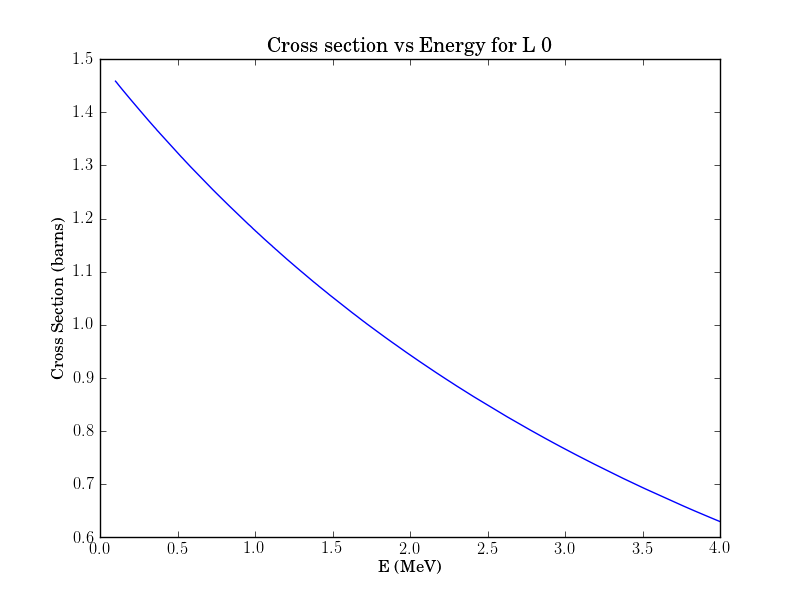
\includegraphics[width=.35\linewidth]{CrossSectionL0}}
\quad
\subfloat{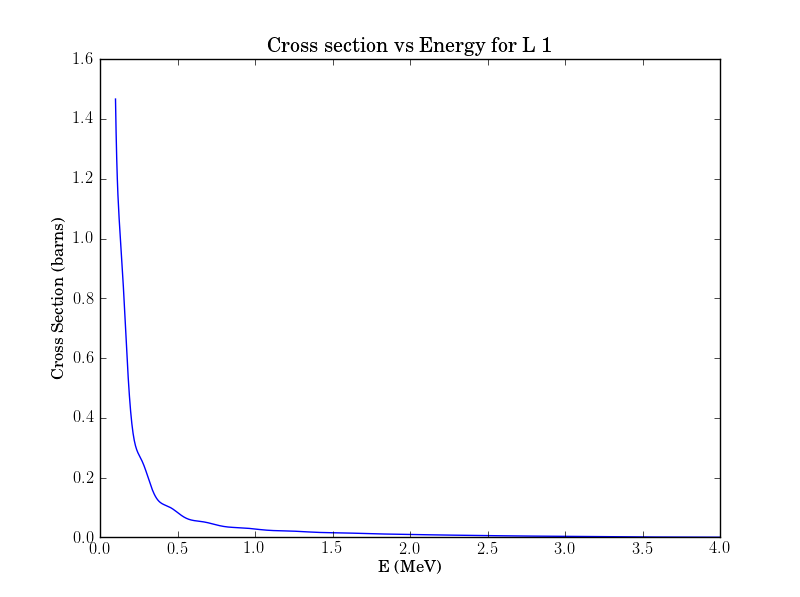
\includegraphics[width=.35\linewidth]{CrossSectionL1}}
\quad
\subfloat{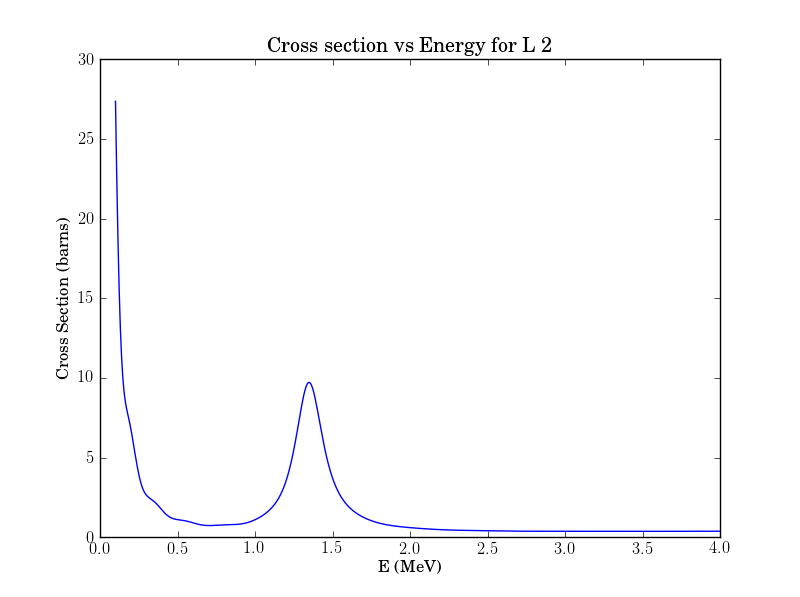
\includegraphics[width=.35\linewidth]{CrossSectionL2}}
\end{floatrow}
\end{figure}
A resonance can be identified as a peak in a plot of cross section against energy, or a sudden rise then leveling off in a plot of phase shift against energy. Based on our results shown in figures above a resonance can be identified for L=2, but not L=0 or L=1. The calculated peak was at 1.345 MeV, which compares favorably with the experimental result of 1.784 MeV. Similarly, the calculated width of the resonance at L=2 is 203 keV. This is in good agreement with the experimental results of the $^{9}$Be(t,p)$^{11}$Be reaction, which had an observed resonance for L=2 with a width of 104 keV. These calculated values were found using the  findpeakinfo method on the data generated from our numerical solutions. 


\section{References}
\begin{enumerate}
\item I. Talmi, I. Unna, Phys. Rev. Lett. 4 (1960) 469
\item G.B. Liu, H.T. Fortune, Phys. Rev. C 42 (1990) 167
\item J.H. Kelley, E. Kwan, J.E. Purcell, C.G. Sheu, H.R. Weller, Nucl. Phys. A 88 (2012) 880
\end{enumerate}


\section{Appendix: Code for generating graphs}
\lstinputlisting{chiscript.py}


\end{document}
